\chapter{Interfaces and Cables}\label{interfaces-and-cables}

SWITCHES provide many PORTS for connectivity (usually 24)

These PORTS tend to be RJ-45 (Registered Jack) ports.

WHAT IS ETHERNET?

\begin{itemize}
\tightlist
\item
  Ethernet is a collection of network protocols/standards.
\end{itemize}

Why do we need network protocols and standards?

\begin{itemize}
\tightlist
\item
  provide common communication standards over networks.
\item
  provide common hardware standards to allow connectivity between
  devices.
\end{itemize}

Connections between devices operates at a set speed.

These speeds are measured in ``bits per second'' (bps)

A bit is a value of ``0'' or ``1''. A byte is 8 bits (0s and 1s)

{\def\LTcaptype{none} % do not increment counter
\begin{longtable}[]{@{}ll@{}}
\toprule\noalign{}
Size & \# of Bits \\
\midrule\noalign{}
\endhead
\bottomrule\noalign{}
\endlastfoot
1 kilobit (Kb) & 1,000 \\
1 megabit (Mb) & 1,000,000 \\
1 gigabit (Gb) & 1,000,000,000 \\
1 terabit (Tb) & 1,000,000,000,000 \\
\end{longtable}
}

Ethernet standards are:

\begin{itemize}
\tightlist
\item
  Defined in the IEEE 802.3 standard in 1983
\item
  IEEE = Institute of Electrical and Electronics Engineers
\end{itemize}

\section{Ethernet Standards (Copper)}\label{ethernet-standards-copper}

{\def\LTcaptype{none} % do not increment counter
\begin{longtable}[]{@{}
  >{\raggedright\arraybackslash}p{(\linewidth - 8\tabcolsep) * \real{0.2000}}
  >{\raggedright\arraybackslash}p{(\linewidth - 8\tabcolsep) * \real{0.2000}}
  >{\raggedright\arraybackslash}p{(\linewidth - 8\tabcolsep) * \real{0.2000}}
  >{\raggedright\arraybackslash}p{(\linewidth - 8\tabcolsep) * \real{0.2000}}
  >{\raggedright\arraybackslash}p{(\linewidth - 8\tabcolsep) * \real{0.2000}}@{}}
\toprule\noalign{}
\begin{minipage}[b]{\linewidth}\raggedright
Speed
\end{minipage} & \begin{minipage}[b]{\linewidth}\raggedright
Common Name
\end{minipage} & \begin{minipage}[b]{\linewidth}\raggedright
Standard
\end{minipage} & \begin{minipage}[b]{\linewidth}\raggedright
Cable Type
\end{minipage} & \begin{minipage}[b]{\linewidth}\raggedright
Max Transmission Distance
\end{minipage} \\
\midrule\noalign{}
\endhead
\bottomrule\noalign{}
\endlastfoot
10 Mbps & Ethernet & 802.3i & 10BASE-T & 100m Max \\
100 Mbps & Fast Ethernet & 802.3u & 100BASE-T & 100m Max \\
1 Gbps & Gigabit Ethernet & 802.3ab & 1000BASE-T & 100m Max \\
10 Gbps & 10 Gigabit Ethernet & 802.3an & 10GBASE-T & 100m Max \\
\end{longtable}
}

BASE = refers to Baseband Signaling

T = Twisted Pair

Most Ethernet uses copper cables.

UTP or Unshielded Twisted Pair (no metallic shield) Twist protects
against EMI (Electromagnetic Interference)

Most use 8 wires (4 pairs) however \ldots{}

10/100BASE-T = 2 pairs (4 wires)

\begin{figure}
\centering
\pandocbounded{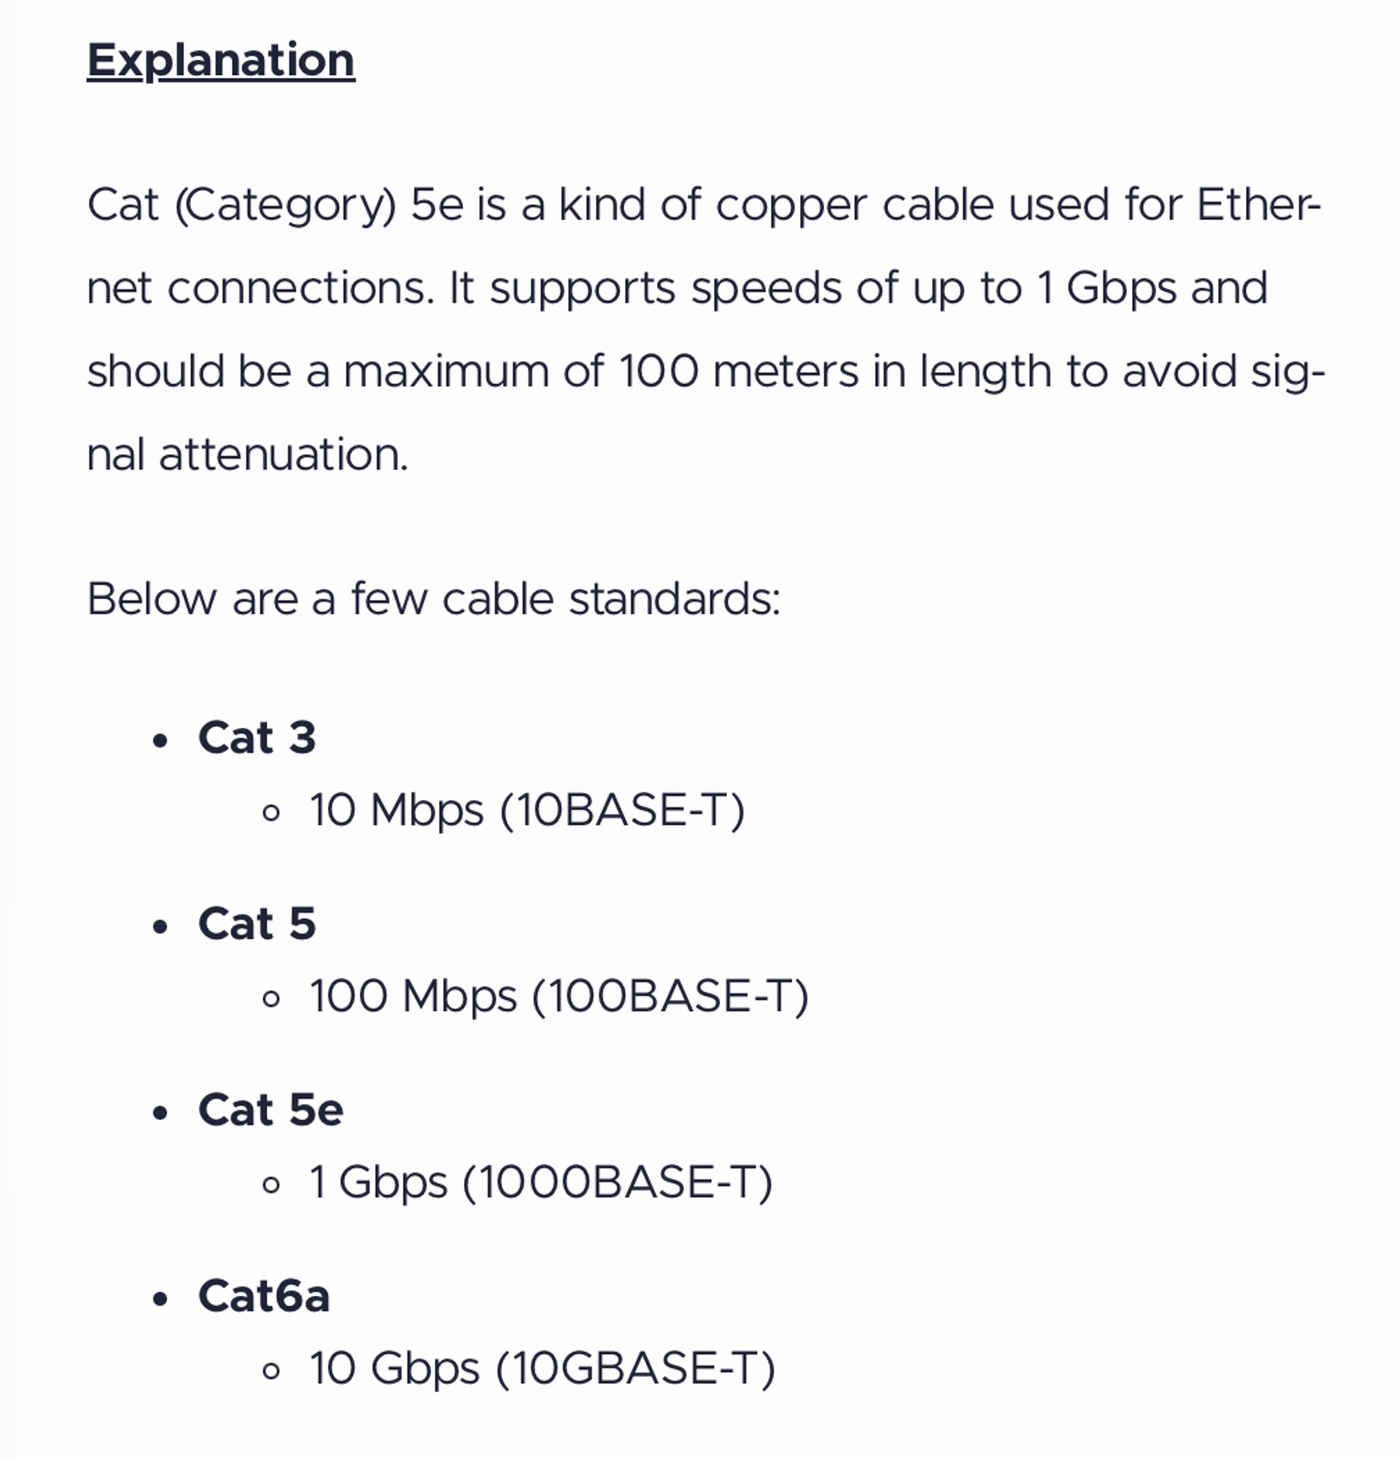
\includegraphics[keepaspectratio,alt={image}]{images/02-interfaces-and-cables/img-001.png}}
\end{figure}

How do devices communicate via their connections?

Each ethernet cable has a RJ-45 plug with 8 pins on the ends.

\begin{figure}
\centering
\pandocbounded{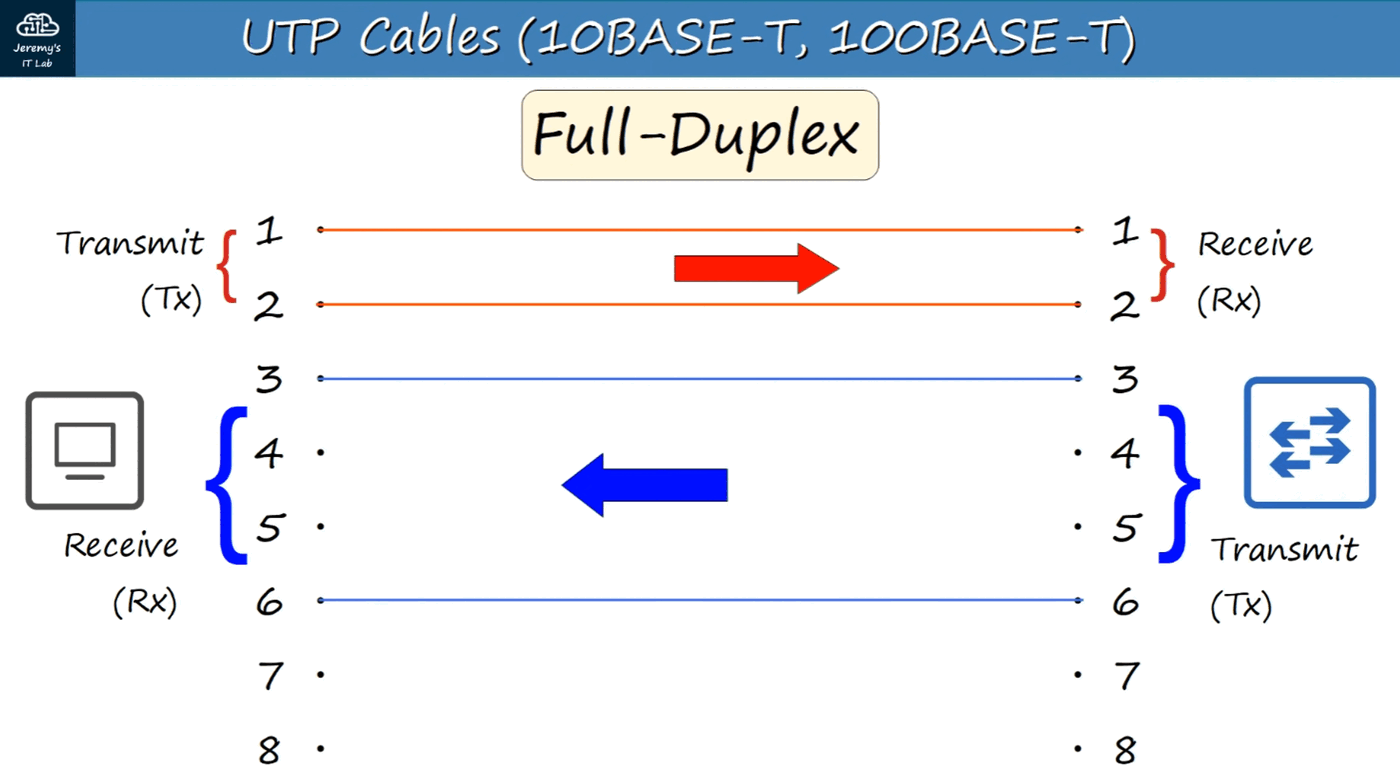
\includegraphics[keepaspectratio,alt={image}]{images/02-interfaces-and-cables/img-002.png}}
\end{figure}

\begin{itemize}
\tightlist
\item
  PCs Transmit(TX) data on Pins \#1-2
\item
  Switches Receive(RX) data on Pins \#1-2
\item
  PCs Receive(RC) data on Pins \#3,6
\item
  Switches Transmit(TX) data on Pins \#3,6
\end{itemize}

This allows Full-Duplex transmission of data.

What if a Router / Switch connect?

\begin{figure}
\centering
\pandocbounded{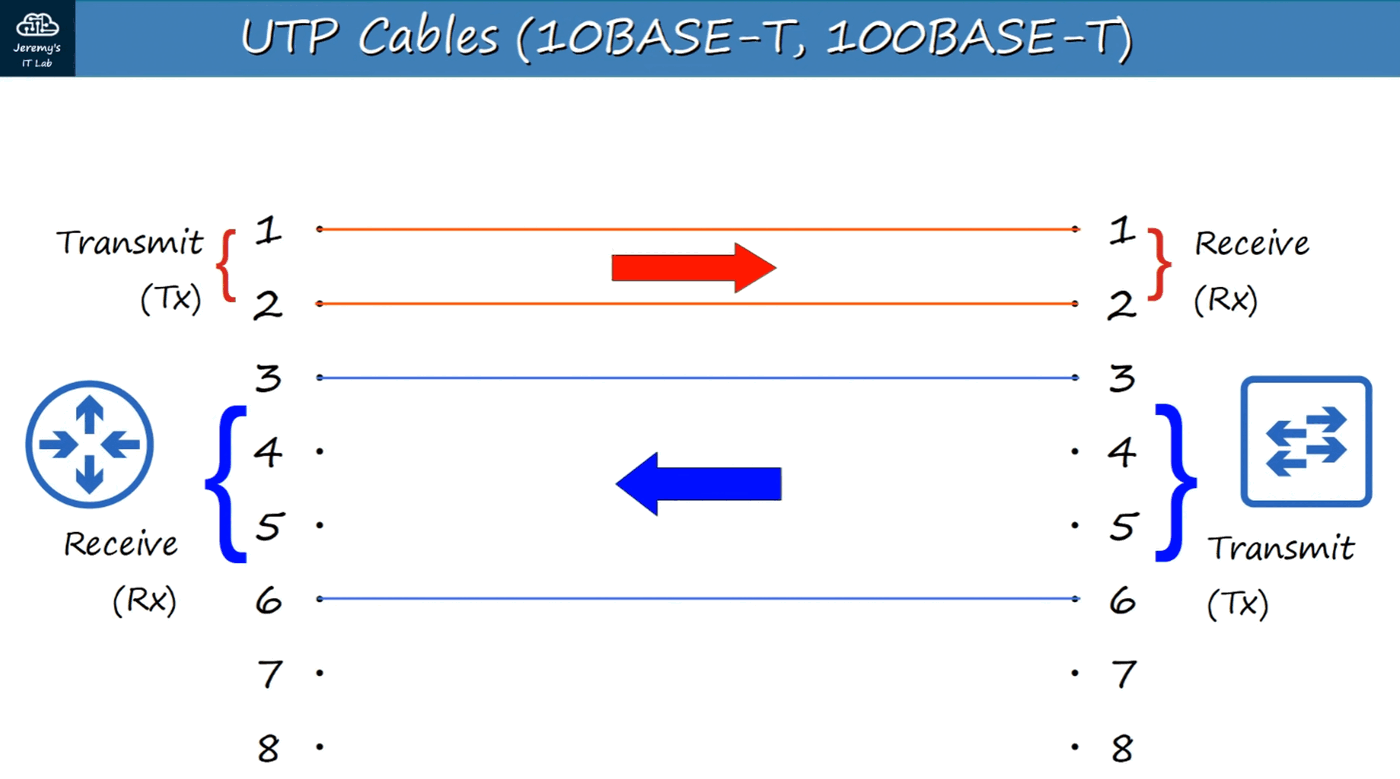
\includegraphics[keepaspectratio,alt={image}]{images/02-interfaces-and-cables/img-003.png}}
\end{figure}

\begin{itemize}
\tightlist
\item
  Routers Transmit(TX) data on Pins \#1-2
\item
  Routers Receive(RX) data on Pins \#3,6
\item
  Switches Transmit(TX) data on Pins \#3,6
\item
  Switches Receive(RX) data on Pins \#1-2
\end{itemize}

Routers and PCs connect the same way with Switches.

The cable used to connect is called a ``Straight-Through'' cable.

What if we want to connect similar devices to each other?

We CANNOT use a ``Straight-Through'' cable. We MUST use a ``Crossover''
cable.

This cable swaps the pins on one end to allow connection to work.

\begin{figure}
\centering
\pandocbounded{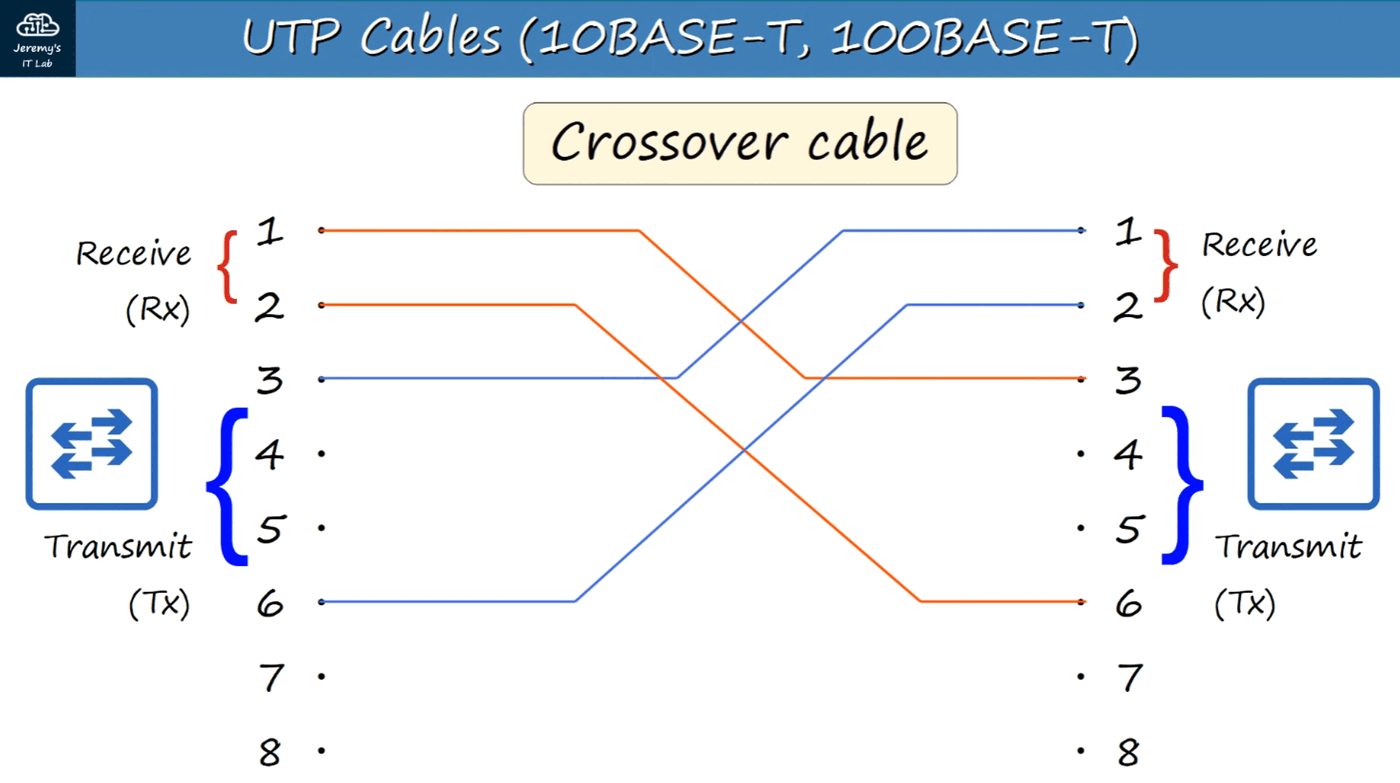
\includegraphics[keepaspectratio,alt={image}]{images/02-interfaces-and-cables/img-004.png}}
\end{figure}

PIN\#1 -----\textgreater{} PIN\#3 PIN\#2 -----\textgreater{} PIN\#6

PIN\#3 -----\textgreater{} PIN\#1 PIN\#6 -----\textgreater{} PIN\#2

{\def\LTcaptype{none} % do not increment counter
\begin{longtable}[]{@{}lll@{}}
\toprule\noalign{}
DEVICE TYPE & TRANSMIT (TX) PINS & RECEIVE (RX) PINS \\
\midrule\noalign{}
\endhead
\bottomrule\noalign{}
\endlastfoot
ROUTER & 1 and 2 & 3 and 6 \\
FIREWALL & 1 and 2 & 3 and 6 \\
PC & 1 and 2 & 3 and 6 \\
SWITCH & 3 and 6 & 1 and 2 \\
\end{longtable}
}

Most modern equipment now has AUTO MDI-X which \textbf{automatically
detects} which pins their neighbour is transmitting on and adjust the
pins they receive data on.

1000BASE-T/10GBASE-T = 4 pairs (8 wires)

Each wire pair is \textbf{bidirectional} so can transmit/receive much
faster than 10/100BASE-T.

\begin{figure}
\centering
\pandocbounded{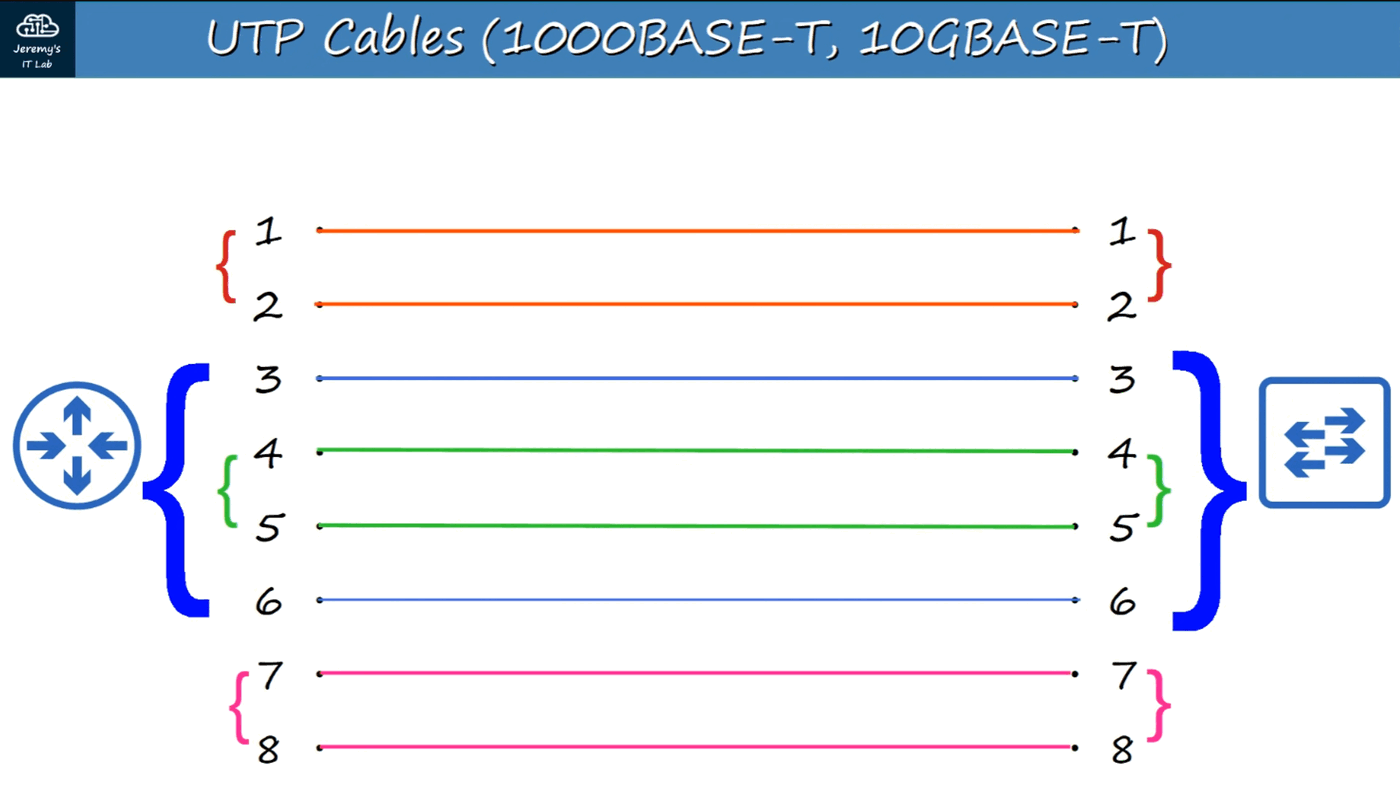
\includegraphics[keepaspectratio,alt={image}]{images/02-interfaces-and-cables/img-005.png}}
\end{figure}

Fiber-Optic Connections:

\begin{itemize}
\tightlist
\item
  Defined in the IEEE 802.3ae standard
\end{itemize}

SFP Transceiver (Small Form-Factor Pluggable) allows fiber-optic cables
to connect to switches/routers.

\begin{itemize}
\tightlist
\item
  Have separate cables to transmit / receive.
\end{itemize}

4 parts to a fiber-optic cable.

\begin{figure}
\centering
\pandocbounded{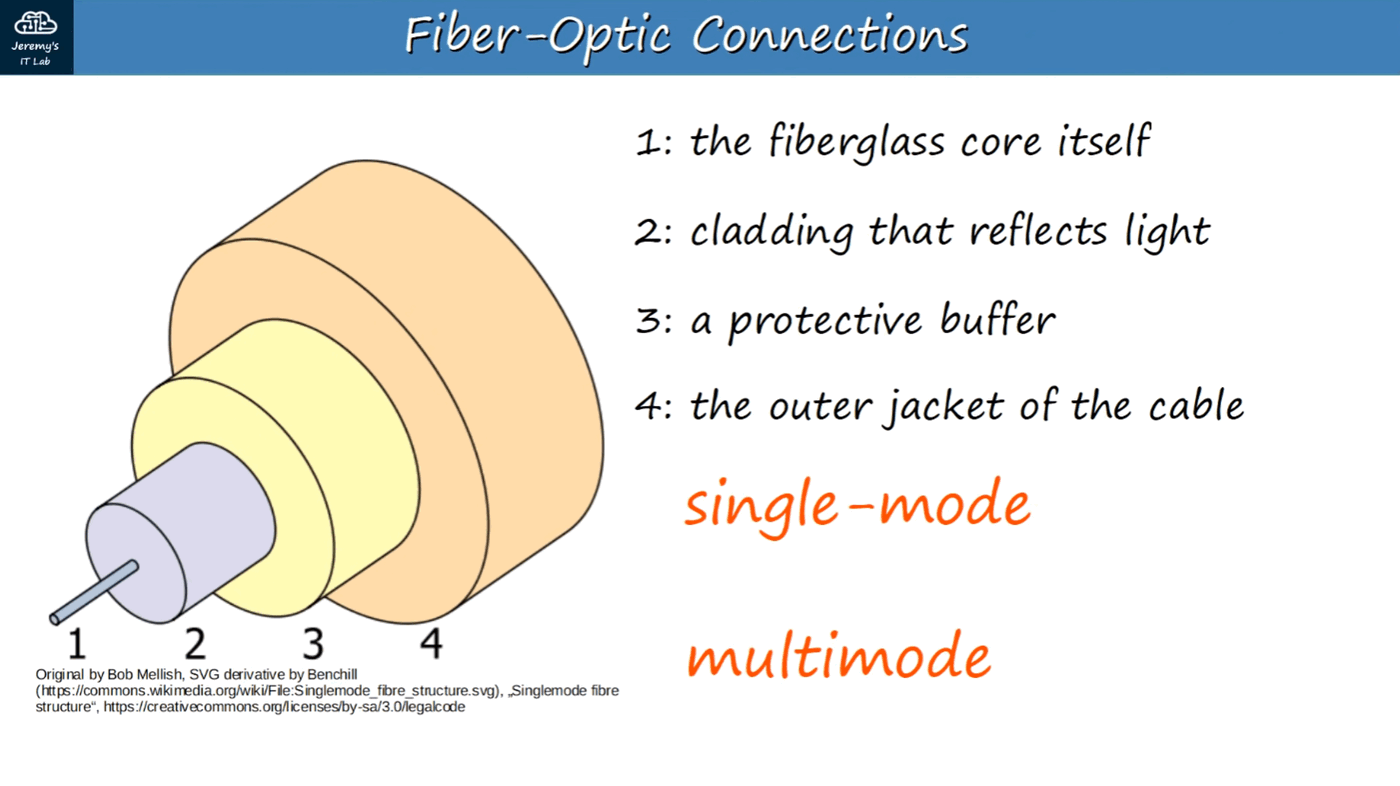
\includegraphics[keepaspectratio,alt={image}]{images/02-interfaces-and-cables/img-006.png}}
\end{figure}

There are TWO types of fiberoptic cable.

Single-Mode:

\begin{figure}
\centering
\pandocbounded{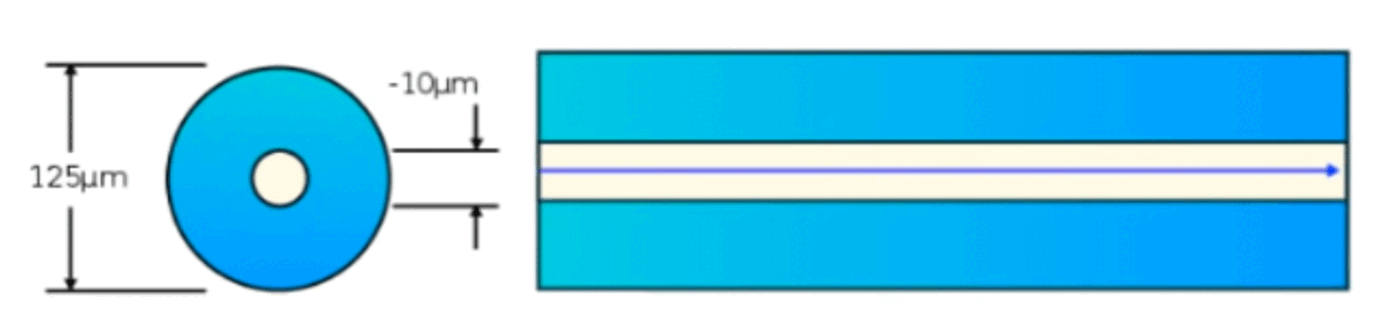
\includegraphics[keepaspectratio,alt={image}]{images/02-interfaces-and-cables/img-007.png}}
\end{figure}

\begin{itemize}
\tightlist
\item
  Narrower than multimode
\item
  Lighter enters at a single angle (mode) from a laser-based
  transmitter.
\item
  Allows longer cables than both UTP and multimode fiber.
\item
  More expensive than multimode fiber (due to more expensive laser-based
  SFP transmitters)
\end{itemize}

Multimode:

\begin{figure}
\centering
\pandocbounded{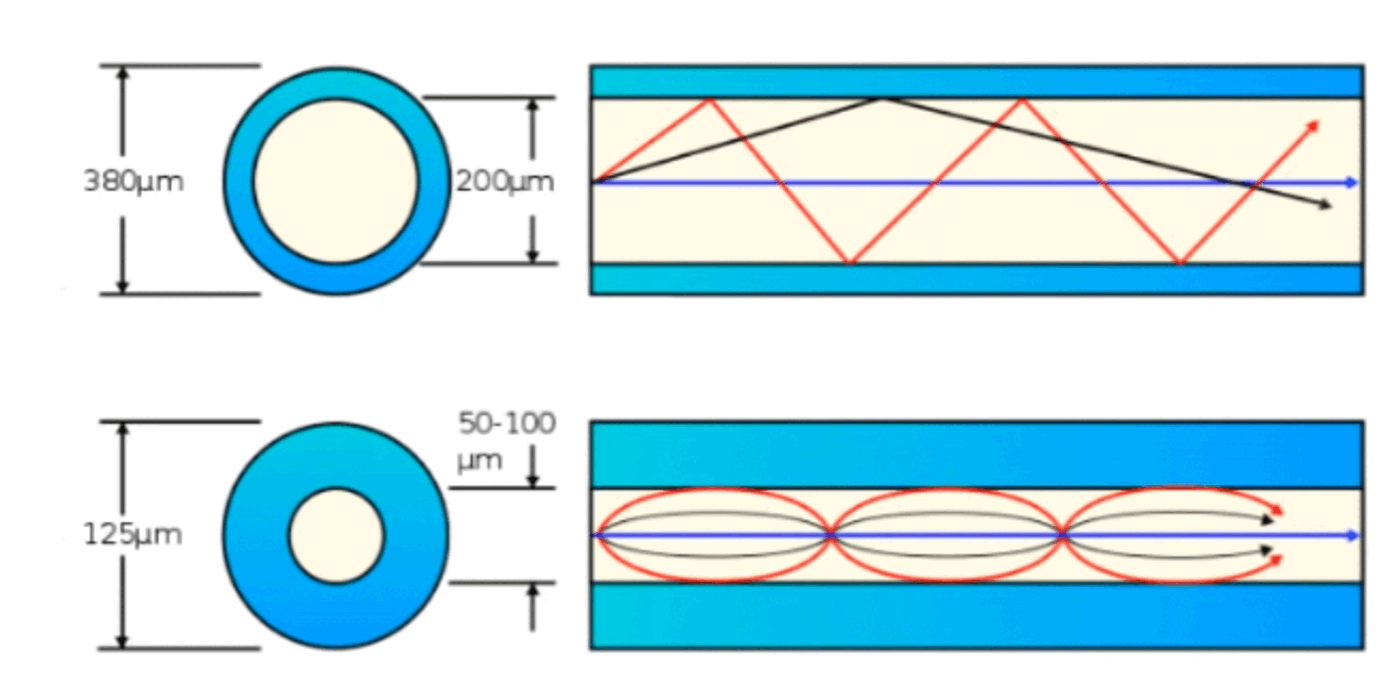
\includegraphics[keepaspectratio,alt={image}]{images/02-interfaces-and-cables/img-008.png}}
\end{figure}

\begin{itemize}
\tightlist
\item
  Core is wider than Single-mode
\item
  Allows multiple angles (modes) of light waves to enter core
\item
  Allows longer cables than UTP but shorter than single-mode
\item
  Cheaper than single-mode fiber (due to cheaper LED-based SFP
  transmitter)
\end{itemize}

Fiber Optic Standards:

{\def\LTcaptype{none} % do not increment counter
\begin{longtable}[]{@{}
  >{\raggedright\arraybackslash}p{(\linewidth - 8\tabcolsep) * \real{0.2000}}
  >{\raggedright\arraybackslash}p{(\linewidth - 8\tabcolsep) * \real{0.2000}}
  >{\raggedright\arraybackslash}p{(\linewidth - 8\tabcolsep) * \real{0.2000}}
  >{\raggedright\arraybackslash}p{(\linewidth - 8\tabcolsep) * \real{0.2000}}
  >{\raggedright\arraybackslash}p{(\linewidth - 8\tabcolsep) * \real{0.2000}}@{}}
\toprule\noalign{}
\begin{minipage}[b]{\linewidth}\raggedright
Speed
\end{minipage} & \begin{minipage}[b]{\linewidth}\raggedright
Standard
\end{minipage} & \begin{minipage}[b]{\linewidth}\raggedright
Connection Speed
\end{minipage} & \begin{minipage}[b]{\linewidth}\raggedright
Mode Support
\end{minipage} & \begin{minipage}[b]{\linewidth}\raggedright
Max Transmission Distance
\end{minipage} \\
\midrule\noalign{}
\endhead
\bottomrule\noalign{}
\endlastfoot
1000BASE-LX & 802.3z & 1 Gbps & Multimode / Single & 550 meters (Multi)
/ 5km (Single) \\
10GBASE-SR & 802.3ae & 10 Gbps & Multimode & 400 meters \\
10GBASE-LR & 802.3ae & 10 Gbps & Single & 10 kilometers \\
10GBASE-ER & 802.3ae & 10 Gbps & Single & 30 kilometers \\
\end{longtable}
}

UTP vs Fiber-Optic Cabling:

UTP are:

\begin{itemize}
\tightlist
\item
  Lower cost than fiber-optic.
\item
  Shorter maximum distance than fiber-optic (\textasciitilde100m).
\item
  Can be vulnerable to EMI (Electromagnetic Interference).
\item
  RJ45 ports used with UTP are cheaper than SFP ports.
\item
  Emit (leak) a faint signal outside of cable, which can be copied
  (security risk).
\end{itemize}

Fiber-Optic:

\begin{itemize}
\tightlist
\item
  Higher cost than UTP.
\item
  Longer maximum distance than UTP.
\item
  No vulnerability to EMI.
\item
  SFP ports are more expensive than RJ45 ports (single-mode is more
  expensive than multimode).
\item
  Does not emit any signal outside of the cable (no security risk).
\end{itemize}
